
%%%%%%%%%%%%%%%%%%%%%%%%%%%  3  %%%%%%%%%%%%%%%%%%%%%%%%%%% 
\subsection{High performance on-chip differential signaling using passive compensation for global communication \cite{zhang2009high}} \label{ss:zhang2009high}
%%%%%%%%%%%%%%%%%%%%%%%%%%%  3  %%%%%%%%%%%%%%%%%%%%%%%%%%% 

\begin{figure}[H]
	\centering
	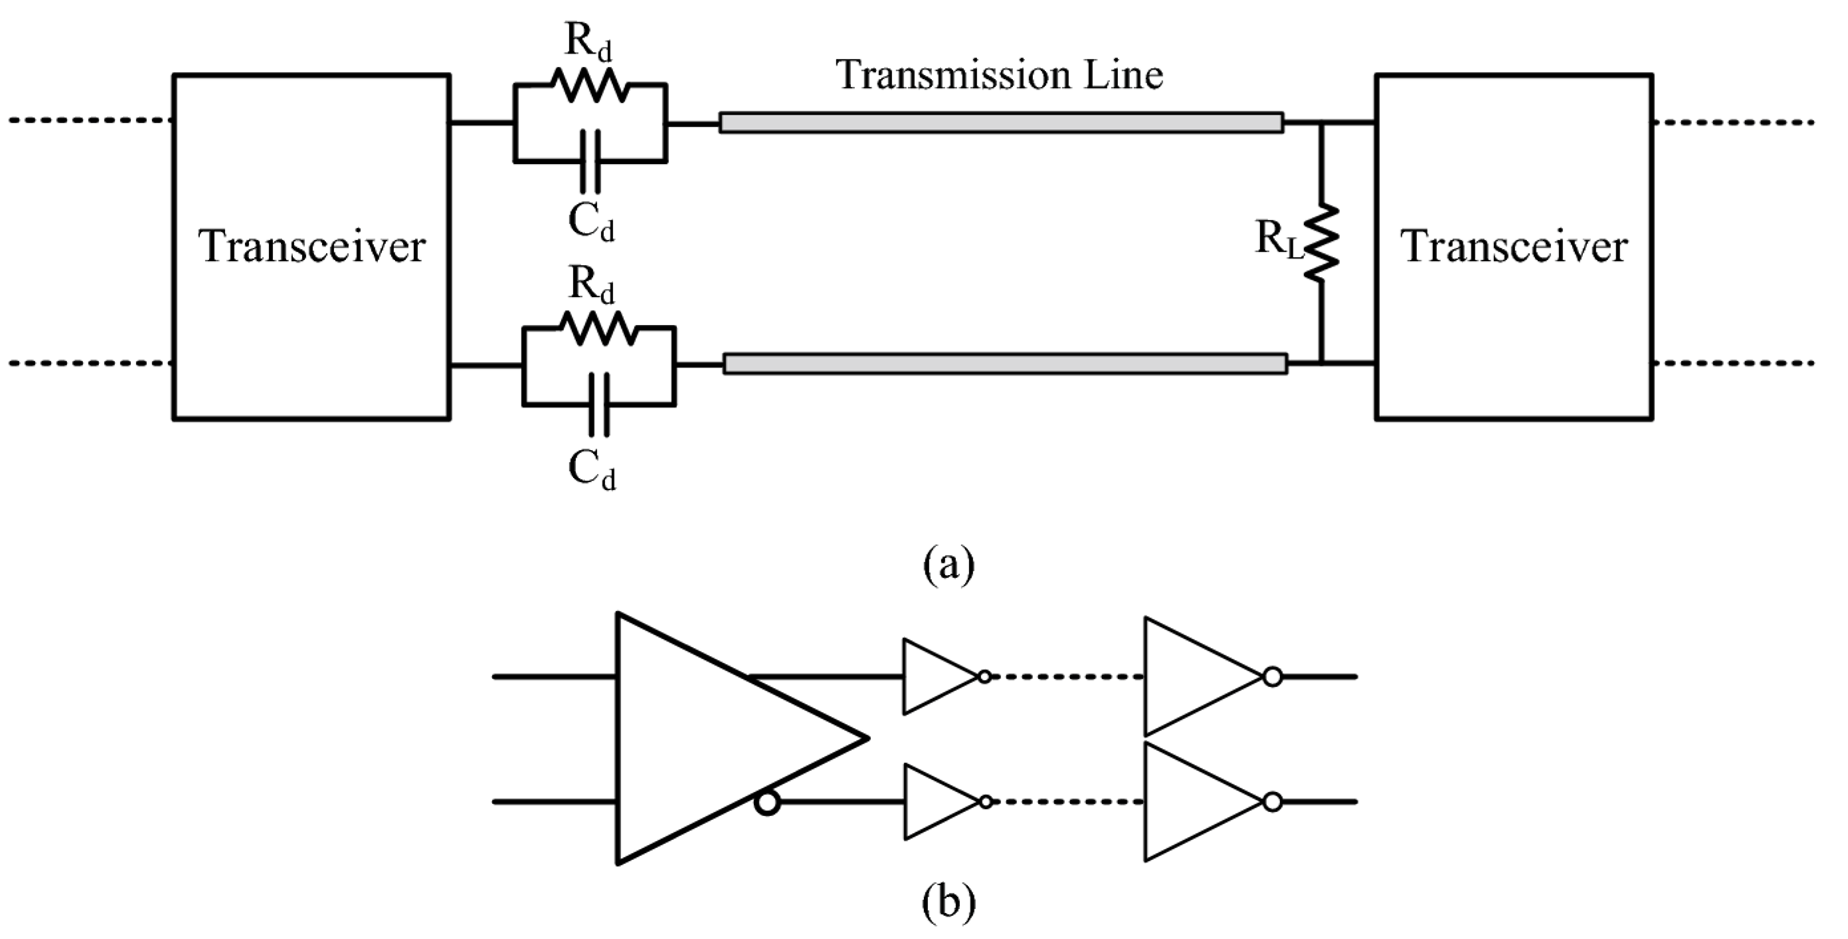
\includegraphics[width=0.95\linewidth]{Figures/Rep3Overview.png}
	\caption{Proposed signaling schema for global wiring: (a) one stage structure; (b) Sense Amplifier + inverter chain structure, Source: \cite{zhang2009high}.} 
    \label{fig:rep3:overview}
\end{figure}

The interconnect of a chip is regarded one of the most critical factors in the determination of performance and power consumption according the ITRS (International Technology Roadmap for Semiconductor) roadmap.
% MISSCHIEN ZIN VERANDEREN DIRECT OVERGENOMEN
For instance, the \textit{1 mm} global RC wire delay (at 45 \textit{nm} technology) is 385 \textit{ps} while the 10 level FO4 delay is below 200 \textit{ps}.
Traditionally the interconnect delay problem is dealed with by implementing a buffer (\textit{buffer insertion} also known as \textit{repeated RC wires}).
However, this introduces a power overhead, i.e. approximately half of the dynamic power is dissipated by the repeaters.

\motive
The use of \accs{otl} deliver signals with speed of light and consumes less power than repeaters, but the \acc{isi} can be a problem for performance.

\objective
A high performance on-chip global signaling with passive compensation is proposed (see \cref{fig:rep3:overview}).
The design is covered and an optimization flow is proposed that optimizes the scheme for a given technology and wire dimension.
Finally the \ac{otl} is compared with repeated RC wires.

\summary
%A. On-Chip T-Line
The proposed signaling schema for global wiring is shown in \cref{fig:rep3:overview}.
For a wire the values of $R_{d}, C_{d} and R_{l}$ determine the eye-opening which are optimized in the optimization flow.

The \ac{otl} is very lossy ($R \neq 0$ and $G \neq 0$) because of the miniaturization of the cross section of the wire.
It can operate in the RC or in the LC region given different frequencies (respectively based on $\omega L \ll R$ (upto 10 GHz) and $\omega L \gg R$).
In LC region the phase velocity and attenuation are independent of frequency.

\begin{figure}
	\centering
	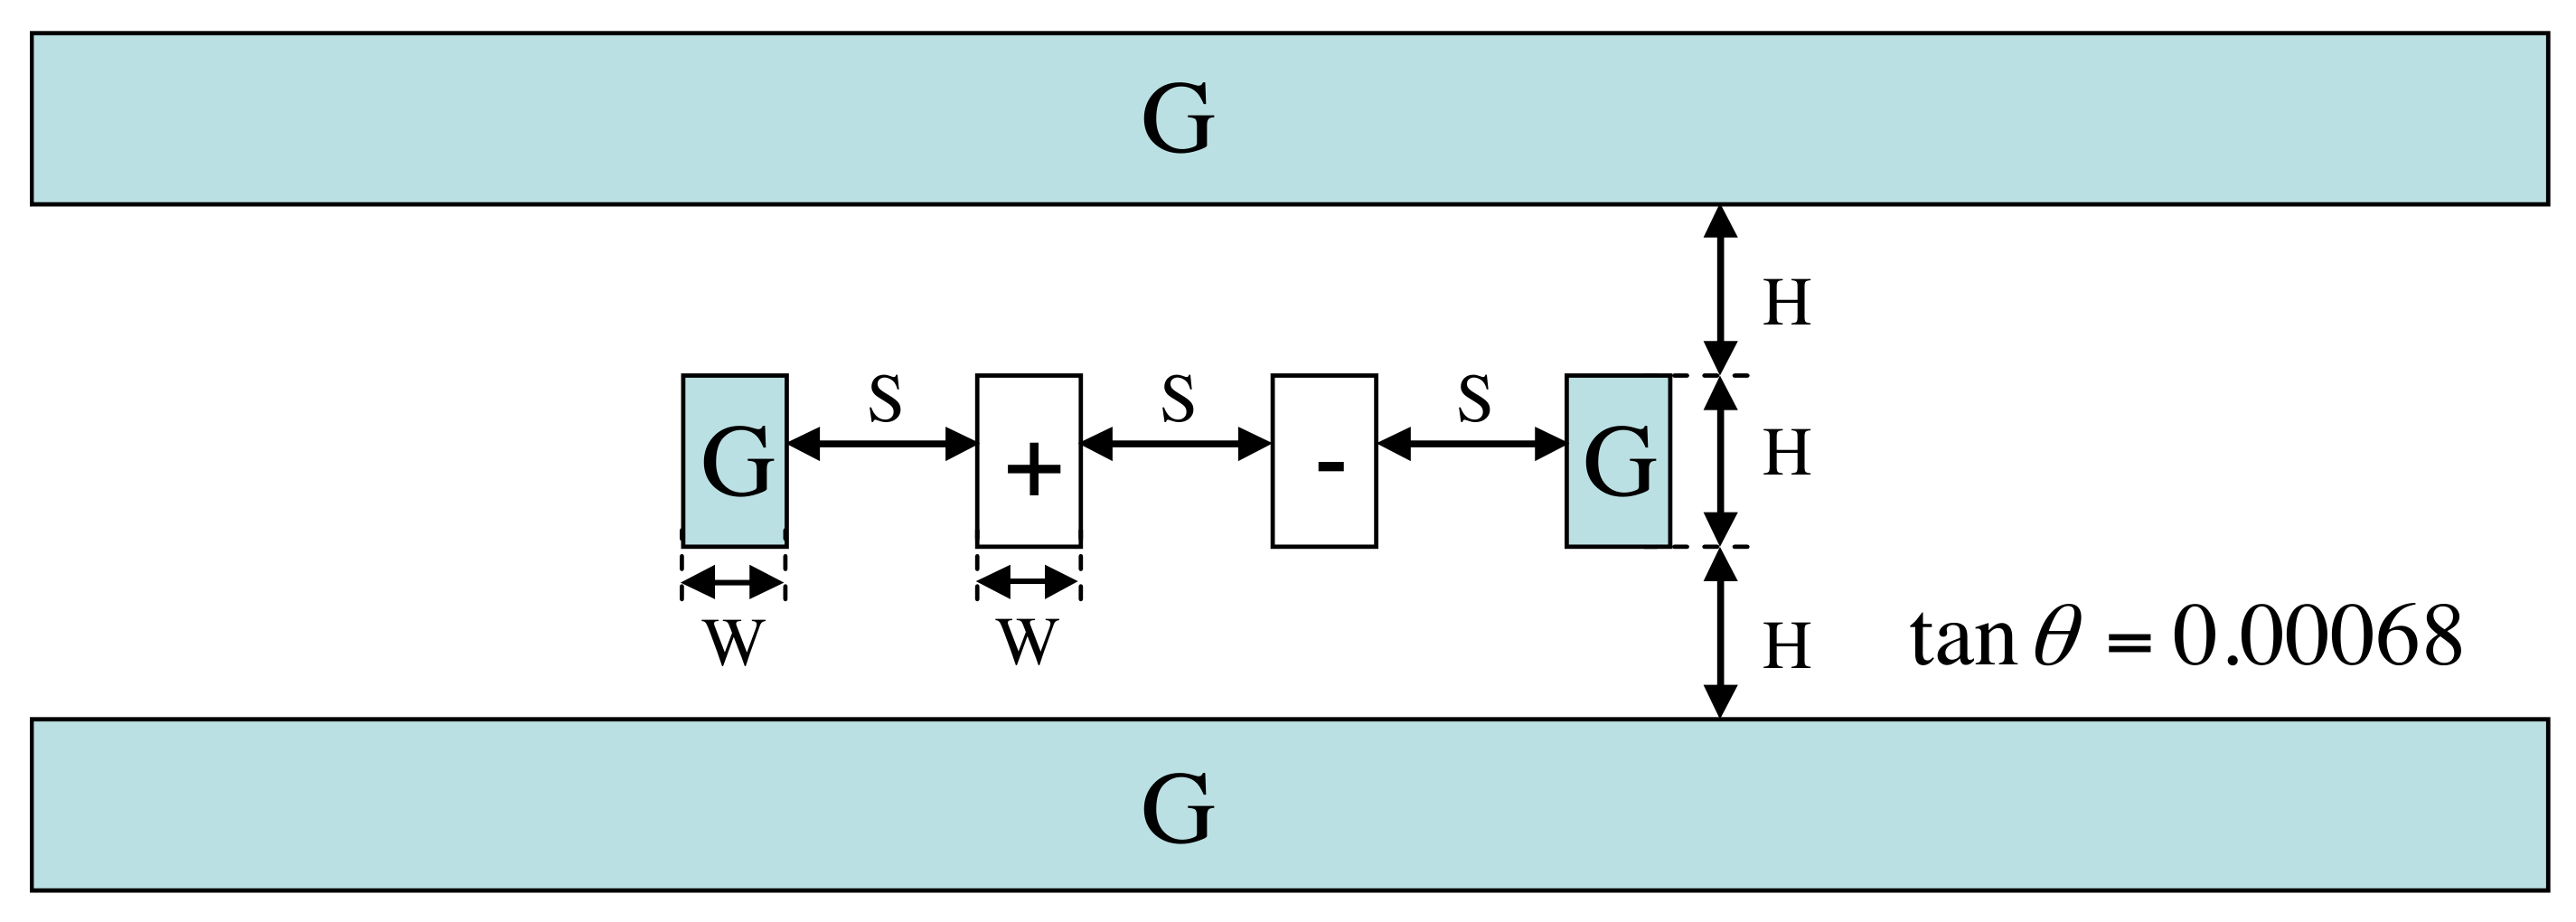
\includegraphics[width=0.95\linewidth]{Figures/Rep3TransmissionLine.png}
	\caption{Cross section of a differential stripline, Source: \cite{zhang2009high}.} 
    \label{fig:rep3:crosssection}
\end{figure}
% Transmission line geometries:
% The length of the global communication in this paper is set to \textit{5 mm}.
According the ITRS roadmap the wire thickness and width ratio should be 2 (see: \cref{fig:rep3:crosssection}).
Larger spacings (S) let the characteristic impedance ($Z_{0}$) increase, which reduces the attenuation and hence gives better eye-diagram performance. %3) Delay and power models ==>> NOT WRITTEN ANYTHING, DO NOT SEE THE USE
% The spacing is varied so that $S = 0.5H, H, 1.5H and 2H$

% B. Transceiver design and modeling
The transceiver stage sense amplifier is based on the same sense amplifier as in \cref{ss:schinkel2009low}.
This design is chosen due to its flexibility to balance the performance metrics.
Simulations have shown that the termination resistance ($R_{l}$) and ($R_{d}$) are dominant in the power consumption.

%Problem formulation and optimization flow


